%
% Sección de BPS. Capítulo de análisis y diseño de generación de tokens
% Proyecto Lovelace.
%

\subsubsection{Algoritmo \textit{BPS}}

La información que aquí se presenta puede ser consultada con mayor detalle en
\cite{bps}.

\textit{BPS} es uno de los algoritmos de cifrado que preservan el formato
existentes, y es capaz de cifrar cadenas de longitudes casi arbitrarias que
estén formadas por cualquier conjunto de caracteres.

\textit{BPS} está conformado por 2 partes fundamentales, un cifrado interno
$BC$, encargado de cifrar bloques de longitud fija; y un modo de operación,
encargado de extender la funcionalidad de el cifrador $BC$ y permitir que
\textit{BPS} cifre cadenas de varias longitudes.

%%%%%%%%%%%%%%%%%%%%%%%%%%%%%%%%%%%%%%%%%%%%%%%%%%%%%%%%%%%%%%%%%%%%%%%%%%%%%%%

\paragraph{El cifrado interno $BC$}

%------------------------------------------------------------------------------

El cifrado por bloques que usa \textit{BPS} internamente se define como
\begin{equation}
  BC_{F,s,b,w}(X,K,T)
\end{equation}

Donde:
\begin{itemize}
  \item $F$ es un cifrador por bloques de $f$ bits de salida,
    por ejemplo: \gls{gl:tdes}, \gls{gl:aes}, \gls{gl:sha}-2.
  \item $s$ es la cardinalidad del conjunto de caracteres del bloque a cifrar.
  \item $b$ es la longitud del bloque a cifrar,
    cumpliendo con $b \leq 2 \cdot |log_s(2^{f-32})|$.
  \item $w$ es el número (par) de rondas de la red Feistel interna
    (véase \ref{sec:red_feistel}).
  \item $X$ es la cadena o bloque de longitud $b$ a cifrar.
  \item $K$ es una llave acorde al cifrador por bloques $F$.
  \item $T$ es un tweak de 64 bits.
\end{itemize}

%------------------------------------------------------------------------------

\textbf(Proceso de cifrado BC.)

Para poder cifrar la cadena $X$:

\begin{enumerate}

  \item Se tiene que dividir el tweak $T$ de 64 bits en 2 subtweaks $T_L$ y
    $T_R$ de 32 bits. Viendo a $T$ como un número entero codificado en binario
    se puede calcular $T_R\: =\: T\: \mod\: 2^{32}$ y
    $T_L\: =\: (T\: -\: T_R) / 2^{32}$

  \item Igualmente, se tiene que dividir en 2 la cadena $X$ para obtener las
    subcadenas $X_L$ y $X_R$ con una longitud $l$ y $r$ respectivamente.
    Dado que la longitud $b$ de la cadena no siempre es par, se tiene que, si
    $b$ es par, entonces tanto $l$ como $r$ son igual a $b/2$, pero en caso
    de que $b$ sea impar, $l$ va a ser igual a $(b+1)/2$ y $r$ igual a
    $(b-1)/2$.

  \item Partiendo de que el cifrador $BC$ se compone de $w$ rondas de una red
    Feistel, se define $L_i$ y $R_i$ (parte izquierda y parte derecha de la
    red en la i-ésima ronda), y se inicializan en:
    \begin{align}
      L_0\: &=\: \sum_{j=0}^{l-1} X_L[j] \cdot s^j \\
      R_0\: &=\: \sum_{j=0}^{r-1} X_R[j] \cdot s^j
    \end{align}

  \item Ahora por cada ronda $i\: <\: w$ y cifrando con el cifrador por
    bloques $E$.

    Si $i$ es par:
    \begin{align}
      L_{i+1}\: &=\: L_i\: \boxplus\:
                    E_K((T_R \oplus i) \cdot 2^{f-32}\: +\: R_i)\qquad
                    (mod\ s^l) \\
      R_{i+1}\: &=\: R_i
    \end{align}

    Si $i$ es impar:
    \begin{align}
      R_{i+1}\: &=\: R_i\: \boxplus\:
                    E_K((T_L \oplus i) \cdot 2^{f-32}\: +\: L_i)\qquad
                    (mod\ s^r) \\
      L_{i+1}\: &=\: L_i
    \end{align}

  \item Por último se tiene que descomponer tanto a $L_w$ como a $R_w$ para
    obtener a $Y_L$ y a $Y_R$ respectivamente, las cuales concatenadas
    ($Y_L \parallel Y_R$) dan la cadena de salida $Y$.

    El proceso para hacer la descomposición se muestra en el pseudocódigo
    \ref{descomposicion_Lw_Rw}.

    \begin{pseudocodigo}[caption={Proceso de descomposición de $L_w$ o $R_w$.},
    label={descomposicion_Lw_Rw}]
      entrada:   bloque $N_w$ de longitud $n$.
      salida:    bloque $Y_N$
      inicio
        para $i=0$ hasta $n-1$
          $Y_N[i] = N_w\ mod\ s$
          $N_w = (N_w - Y_N[i])/s$
      fin
    \end{pseudocodigo}

\end{enumerate}

De forma general, el proceso de cifrado se describe en el pseudocódigo
\ref{cifrado_BC}.

%Pseudocodigo excediéndose de los 80 para una correcta visualización el en pdf ---------------------------
\begin{pseudocodigo}[caption={Proceso de cifrado $BC$.},
label={cifrado_BC}]
  entrada:    la llave $K$, el tweak $T$, la cadena $X$ de longitud $b$ formada por el conjunto $S$
              de cardinalidad $s$, la función de cifrado $F$, y el número de rondas $w$.
  salida:     La cadena cifrada $Y$.
  inicio
    calcular $T_R\: =\: T\: \mod\: 2^{32}$ y $T_L\: =\: (T\: -\: T_R) / 2^{32}$
    asignar $l = r = b/2$
    inicializar $L_0\: =\: \sum_{j=0}^{l-1}\: X[j] \cdot s^j$
    inicializar $R_0\: =\: \sum_{j=0}^{r-1}\: X[j+l] \cdot s^j$
    para $i=0$ hasta $i=w-1$
      si $i$ es par
        $L_{i+1}\: =\: L_i\: \boxplus\: F_K((T_R \oplus i) \cdot 2^{f-32}\: +\: R_i)\qquad (mod\ s^l)$
        $R_{i+1}\: =\: R_i$
      si $i$ es impar
        $R_{i+1}\: =\: R_i\: \boxplus\: F_K((T_L \oplus i) \cdot 2^{f-32}\: +\: L_i)\qquad (mod\ s^r)$
        $L_{i+1}\: =\: L_i$
    para $i=0$ hasta $i=l-1$
      $Y_L[i] = L_w\ mod\ s$
      $L_w = (L_w - Y_L[i])/s$
    para $i=l$ hasta $i=r-1$
      $Y_R[i] = R_w\ mod\ s$
      $R_w = (R_w - Y_R[i])/s$
    determinar $Y = Y_L \parallel Y_R$
  fin
\end{pseudocodigo}
%Pseudocodigo excediéndose de los 80 para una correcta visualización el en pdf ---------------------------

%------------------------------------------------------------------------------

\textbf(Proceso de descifrado $BC^{-1}$.)

Para poder descifrar la cadena $Y$:

\begin{enumerate}

  \item Se tiene que dividir en 2 la cadena $Y$, para obtener las subcadenas
    $Y_L$ y $Y_R$ con una longitud $l$ y $r$ respectivamente, de igual forma
    que se hizo con la cadena $X$ en el proceso de cifrado.

  \item Partiendo de que el proceso de descifrado se compone de $w$ rondas,
    se define $L_i$ y $R_i$ y se inicializan en:
    \begin{align}
      L_w\: &=\: \sum_{j=0}^{l-1} Y_L[j] \cdot s^j \\
      R_w\: &=\: \sum_{j=0}^{r-1} Y_R[j] \cdot s^j
    \end{align}

  \item Ahora, comenzando con $i=w-1$, para cada ronda $i\: \geq\: 0$.

    Si $i$ es par:
    \begin{align}
      L_i\: &=\: L_{i+1}\: \boxminus\:
                E_K((T_R \oplus i) \cdot 2^{f-32}\: +\: R_{i+1})\qquad
                (mod\ s^l) \\
      R_i\: &=\: R_{i+1}
    \end{align}

    Si $i$ es impar:
    \begin{align}
      R_i\: &=\: R_{i+1}\: \boxminus\:
                E_K((T_L \oplus i) \cdot 2^{f-32}\: +\: L_{i+1})\qquad
                (mod\ s^r) \\
      L_i\: &=\: L_{i+1}
    \end{align}

  \item Finalmente se tienen que descomponer $L_0$ y $R_0$ (con el mismo
    proceso de descomposición descrito en el cifrado) para obtener a $X_L$ y
    $X_R$, las cuales concatenadas ($X_L \parallel X_R$) dan la cadena de
    salida $X$.

\end{enumerate}

De forma general, el proceso de descifrado se describe en el pseudocódigo
\ref{descifrado_BC}.

%Pseudocodigo excediéndose de los 80 para una correcta visualización el en pdf ---------------------------
\begin{pseudocodigo}[caption={Proceso de descifrado $BC^{-1}$.},
label={descifrado_BC}]
  entrada:    la llave $K$, el tweak $T$, la cadena $Y$ de longitud $b$ formada por el conjunto $S$
              de cardinalidad $s$, la función de cifrado $F$, y el número de rondas $w$.
  salida:     La cadena $X$.
  inicio
    calcular $T_R\: =\: T\: \mod\: 2^{32}$ y $T_L\: =\: (T\: -\: T_R) / 2^{32}$
    asignar $l = r = b/2$
    inicializar $L_w\: =\: \sum_{j=0}^{l-1}\: Y[j] \cdot s^j$
    inicializar $R_w\: =\: \sum_{j=0}^{r-1}\: Y[j+l] \cdot s^j$
    para $i=w-1$ hasta $i=0$
    si $i$ es par:
      $L_i\: =\: L_{i+1}\: \boxminus\: F_K((T_R \oplus i) \cdot 2^{f-32}\: +\: R_{i+1})\qquad (mod\ s^l)$
      $R_i\: =\: R_{i+1}$
    si $i$ es impar:
      $R_i\: =\: R_{i+1}\: \boxminus\: F_K((T_L \oplus i) \cdot 2^{f-32}\: +\: L_{i+1})\qquad (mod\ s^r)$
      $L_i\: =\: L_{i+1}$
    para $i=0$ hasta $i=l-1$
      $X_L[i] = L_w\ mod\ s$
      $L_w = (L_w - X_L[i])/s$
    para $i=l$ hasta $i=r-1$
      $X_R[i] = R_w\ mod\ s$
      $R_w = (R_w - X_R[i])/s$
    determinar $X = X_L \parallel X_R$
  fin
\end{pseudocodigo}
%Pseudocodigo excediéndose de los 80 para una correcta visualización el en pdf ---------------------------

%%%%%%%%%%%%%%%%%%%%%%%%%%%%%%%%%%%%%%%%%%%%%%%%%%%%%%%%%%%%%%%%%%%%%%%%%%%%%%%

\paragraph{El modo de operación}

En cuanto al modo de operación de \textit{BPS}, se puede decir que es un
equivalente al modo de operación CBC (véase \ref{sec:cbc}), ya que el bloque
$BC_n$ utiliza el texto cifrado de la salida del bloque $BC_{n-1}$, con la
distinción de que en lugar de aplicar operaciones \textit{xor} usa sumas
modulares carácter por carácter, y de que no utiliza un
\gls{gl:vector_de_inicializacion}, a pesar de soportar su uso.

Algo importante a resaltar de este modo de operación es que, en caso de que el
texto en claro no tenga una longitud total que sea múltiplo de la longitud de
bloque $b$, al cifrar el último bloque se recorre el cursor que determina
el inicio del mismo, hasta que su longitud concuerde con $b$, esto se puede
ver de forma gráfica en la figura \ref{cursor_BPS}.

\begin{figure}[H]
  \begin{center}
    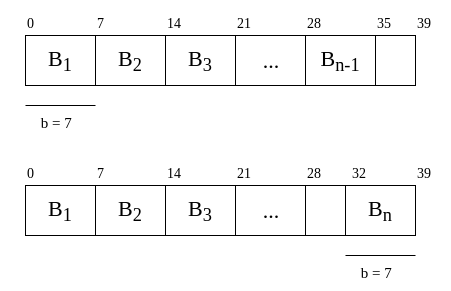
\includegraphics[width=0.5\linewidth]
    {../../../../../diagramas_comunes/bps/cursor_bps}
    \caption{Ejemplo del corrimiento de cursor para la selección del ultimo
      bloque en el modo de operación de \textit{BPS}.}
    \label{cursor_BPS}
   \end{center}
\end{figure}

En la figura \ref{modo_de_operacion_BPS} se ve de manera gráfica el
funcionamiento del modo de operación de \textit{BPS}.

\begin{figure}[H]
  \begin{center}
    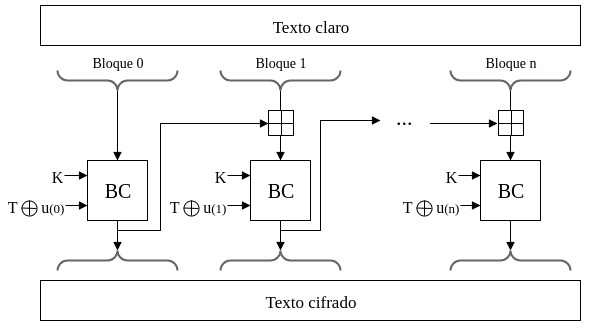
\includegraphics[width=0.85\linewidth]
    {../../../../../diagramas_comunes/bps/modo_de_operacion_bps}
    \caption{Modo de operación de \textit{BPS}.}
    \label{modo_de_operacion_BPS}
   \end{center}
\end{figure}

Otra particularidad del modo de operación es el uso del contador $u$ de 16
bits, que es utilizado para aplicar una operación \textit{xor} al tweak $T$
que entra a cada uno de los bloques $BC$. Recordando que $T$ es de 64 bits,
el \textit{xor} se aplica a los 16 bits más significativos de ambas mitades
de tweak, esto debido a cada mitad de tweak funciona de manera independiente
en el cifrador $BC$, y a que no se desea un traslape entre el contador externo
$u$ y el contador $i$ interno en $BC$.

%%%%%%%%%%%%%%%%%%%%%%%%%%%%%%%%%%%%%%%%%%%%%%%%%%%%%%%%%%%%%%%%%%%%%%%%%%%%%%%

\paragraph{Características generales}

Como se observó, \textit{BPS} está basado en las redes Feistel, lo cual puede
verse como una ventaja, debido al amplio estudio que tienen. Además, usa
algoritmos de cifrado o funciones hash estandarizadas de forma interna, lo
cual hace más comprensible y fácil su implementación.

\textit{BPS} es un cifrado que preserva el formato capaz de cifrar cadenas de
un longitud de $2$ hasta $max(b) \cdot 2^{b}$ caracteres (donde $max(b)$ es el
tamaño máximo de bloque), formadas por cualquier conjunto.

Se puede considerar que \textit{BPS} es eficiente, debido a que la llave $K$
usada en cada bloque $BC$ es constante, y a que además usa un número reducido
de operaciones internas en comparación con otros algoritmos de cifrado que
preservan el formato.

Por último, se puede resaltar que el uso de tweaks protege a \textit{BPS} de
ataques de diccionario, los cuales son fáciles de cometer cuando el dominio
de la cadena a cifrar es muy pequeño.

%%%%%%%%%%%%%%%%%%%%%%%%%%%%%%%%%%%%%%%%%%%%%%%%%%%%%%%%%%%%%%%%%%%%%%%%%%%%%%%

\paragraph{Recomendaciones}

Se recomienda que el número de rondas $w$ de la red Feistel sea $8$, dado
que es una número de rondas eficiente, y se ha estudiado la seguridad de
\textit{BPS} con este $w$.

Es recomendable que como tweak se use la salida truncada de una función hash,
en donde la entrada de la función puede ser cualquier información relacionada
a los datos que se deseen proteger, como por ejemplo fechas, lugares, o parte
de los datos que no se deseen cifrar.
